\section{Text Normalisation Techniques}
\label{sec-background}

\subsection{Text Pruning}
This raw text of $train.txt$ and $dev.txt$ provides us with our first problem. We need to transform our raw text data into a set of features that describe qualitative concepts in a quantitative way, we call this as feature vector space. In our case, that will be a 1/-1 coding strategy: Yes or No. For the this project, we process our features such that they do not include words beginning with {\#} and {$@$} and we are more concerned with English words. We use {\citet{gm14}} for text normalisation.



\subsection{Feature Engineering}
Before we begin analysing our tokens, we would want to categorise and extract the tokens which we would want to consider as attributes. Our focus is to combine attributes into various n- gram categories, such as 1 Gram, 2 Gram, 3 Gram; defining them as non-gram attributes. We use $tokens.txt$ and $dev.txt$ for extracting the attributes. We maintain the token in a line-by-line format in $N$$-$$gramtoken.txt$, where ${N=1,2,3}$. This is perform in the $n-gram.py$ where we can pass N as a parameter and the script returns a feature vector space of the entire file that is being parsed. 

Feature subset selection is the process of identifying and removing as many irrelevant and redundant features as possible. This reduces the dimensionality of the data and enables data mining algorithms to operate faster and more effectively.
For this we apply \textbf{LASSO} ({least absolute shrinkage and selection operator}) and we make an interesting observation. 

In our observation {neck, pic, skin, restless and zombie} can produce quite a high number of correctly classified instances. To put things in perspective, using the Support vector machine, we received 82.15\% correctly classified instances when classifying $dev$ keeping $train$ as the prepossessing module, while just using particularly these 5 words gives us a staggering, 89.68 \% correctly classified instances and 10.316 \% incorrectly classified instances. The other parameters such as root mean square error and relative absolute error also take a substantial decrease above 45\%.However, it is quite obvious that these 5 features alone may not be sufficient for us to classify the unknown $test$ classes and we need some number of instances. However, this observation tells us something about the data i.e. there is a clear bias in the weightage each of the 92 attribute has and perhaps identifying the key attributes can help us in forming new set of attributes. 

We further explore the 'Select attributes' tab in the $WEKA$ explorer, this will allow us to explore rankings the attributes. There are two parameters to observe here $attribute evaluator$ and $search method$. We start with exploring the $InfoGainAttributeEval$ which evaluates the worth of attribute by measuring the information gain with respect to the class. We use $GreedyStepwise$ for the search method, which uses the greedy algorithm for ranking attributes. A threshold greater than 0.0050 is chosen; An overview of the attributes is shown in \textbf {Table 2}.  

Lastly, we explore synonyms of words and search for approximate matching words using dictionary. Note: we only record those tokens which exists in our twitter files. Using the all the above approaches we get a 3-gram, 48 line token file as our feature selection. 

\begin{table}[t]
\centering

 \begin{tabular}{|c|c|} 
 \hline
 Corpus & Features \\ [0.5ex] 
 \hline\hline
 train.arff & 639KB-3166 tweets \\ 
\hline
dev.arff & 219KB-1076 tweets \\
 \hline
 test.arff & 221 KB-1087 tweets \\
 \hline
\end{tabular}
\mycaption{Corpura used for identifying tweets with ADR
\label{tbl-normalize}}
\aftertabspace
\end{table}

 
\subsection{{\itshape Classification} Techniques}
  
 When classification is to be performed, we have to seperate data into training and testing sets. Each instance in the training set contains one 'target value' (i.e. the class labels) and several 'attributes' (i.e. the features or observed variables). 
 
 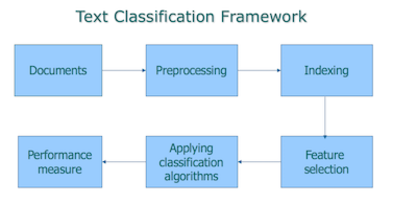
\includegraphics {finalgraph8.pdf}
  
\textbf{Naive Bayes Classification Technique:} Naive Bayes classifier, looks for differences of this sort by searching through text for words that are either (a) noticeably more likely to occur in A class, or (b) noticeably more likely to occur in B class. When a word is noticeably more likely to occur in one context rather than the other, its occurrence can be diagnostic of whether a new message is in A or B. If we see a single word that's more likely to occur in A than B, that's evidence that the token as a whole is in class A. 

Quite evidently, this approach is quite east of implement. Decent results are returned from this technique.

\textbf{Support Vector Machine:} The goal of Support vector machine (SVM for short) is to produce a model (based on the training data) which predicts the target values of the test data given only the test data attributes. SVM finds a linear separating hyperplane with the maximal margin. The instances that are closest to the maximum hyperplane are called support vectors. 

The kernel trick that could be used to solve problems with nonlinear decision boundaries. SVM allows you to use multiple different kernels to find nonlinear decision boundaries. 

\textbf{Decision Trees:} The root node in decision tree contains all the documents. Each internal node is a subset of documents separated by one attribute. Each node is further labelled with a predicate which can be applied at the parent. Finally, each leaf node is labelled with a class.Through the decision tree we were able get an accuracy of 

The confidence is used to compute the pessimistic upper bound of the error rate and is higher for pruning. J48 does not accept values greater then 0.5. 

\textbf{} 

\textbf{Perceptron(a review):} 
We use sklearn and numpy to develop a perceptron model as it is a binary classifier. We do this on just our tokens and try to understand the relation between testing and training errors. Further we adjust parameters such as the learning rate (eta). We observe that lower the learning rate higher the training accuracy. We receive an accuracy of 88.97\% on our training set. The average test error computes to 0.16\% and train error is 0.12\%. This process is performed on the basis of heldout validation. Perceptron is introduced as an alternative to existing approaches and can be explored further in future studies. 


   
\begin{table}[t]
\centering

 \begin{tabular}{c c c c} 
 \hline
 Character & Word position-Word \\ [0.5ex] 
 \hline\hline
 0.01235 & 50-me\\ 

 0.01079 & 48-makes\\

 0.00924  & 29-feel\\
 
 0.00883 & 40-i \\ 

 0.00836 & 46-lozenge \\

 0.00688 & 76-sick\\

 0.00655 & 67-prozac \\
 
 0.00638 & 42-it\\ 

 0.00621 & 49-making\\

 0.00619 & 63-pain\\

 0.00598 & 61-olanzapine\\
 
 0.00591 & 32-gain\\

 0.00587 & 93-zombie\\
 
 0.00543 & 89-weight \\ 

 0.00510 & 65-person\\

 \hline
\end{tabular}

\mycaption{Select Attributes 
\label{tbl-normalize}}
\aftertabspace
\end{table}





\subsection{Comparison and Review}
\label{sec-somethingnew}

\begin{table*}[t]
\centering
\begin{center}
 \begin{tabular}{c c c c c} 
 \toprule
 Type
 	& Correctly classified instances
		& Precisson
			& Recall
				& F-Measure
\\ 
 \midrule
Zero-R
 	& 89.4052\%
		& 0.799
			& 0.894
				& 0.844
 \\
 Naive Bayes
 	& 82.1561\%
		& 0.866
			& 0.822
			& 0.840
			 \\ 

 Decision Tree(J48) 
 	& 89.3123\% & 0.860 & 0.893 & 0.864\\
	
 Random Forest
 	& 89.4052\% & 0.860 & 0.894 & 0.861\\	
%% Requirements
%% 	& 	&  & Dependent \\ 
 
 Support Vector Machines
 	& 89.5911\%
		& 0.866
			& 0.896
			& 0.865
\\

 \bottomrule
\end{tabular}
\end{center}
\mycaption{Performance comparison of classification strategies without new tokens
\label{tbl-normalize}}
\aftertabspace
\end{table*}

\begin{table*}[t]
\centering
\begin{center}
 \begin{tabular}{c c c c c} 
 \toprule
 Type
 	& Correctly classified instances
		& Precisson
			& Recall
				& F-Measure
\\ 
 \midrule
Zero-R
 	&  89.4052\%
		& 0.799
			& 0.894
				& 0.844
 \\
 Naive Bayes
 	&  82.1561\%
		& 0.866
			& 0.822
			& 0.840
			 \\ 

 Decision Tree(J48) 
 	& 89.5911\% & 0.866 & 0.896 & 0.867\\
	
 Random Forest
 	& 89.5911\% & 0.865 & 0.896 & 0.858\\	
%% Requirements
%% 	& 	&  & Dependent \\ 
 
 Support Vector Machines
 	& 90.0558\%
		& 0.878
			& 0.901
			& 0.871
\\

 \bottomrule
\end{tabular}
\end{center}
\mycaption{Performance comparison of classification with new tokens
\label{tbl-normalize}}
\aftertabspace
\end{table*}
  


An overview of the attributes is shown in \textbf {Table 3} and \textbf{Table 4}.
Accuracy is computed as in equation  \eqref{eq:accuracy}.

\begin{equation}
\label{eq:accuracy}
Accuracy = \frac{\mathit{Total\ correct\ predictions}}{\mathit{Number\ of\ test\ predictions}}
\end{equation}


Precision is computed as in equation \eqref{eq:precision}.

\begin{equation}
\label{eq:precision}
Precision = \frac{\mathit{Number\ of\ correct\ predictions}}{\mathit{Total\ number\ of\ predictions}}
\end{equation}

Recall is computed as in equation \eqref{eq:recall}.

\begin{equation}
\label{eq:recall}
Recall = \frac{\mathit{Number\ of\ correct\ words}}{\mathit{Total\ number\ of\ words}}
\end{equation}

F-measure is computed as in equation  \eqref{eq:fmeasure}.

\begin{equation}
\label{eq:fmeasure}
F-Measure = \frac{\mathit{2\ *\ Precision\ *\ Recall}}{\mathit{Precison\ +\ Recall}}
\end{equation}

\myparagraph{Naive Bayes} The low accuracy rate can be attributed to the assumption of class conditional independence. As we know that in practical systems, there is a dependency between variables. We were unable to find a way of modelling these dependencies directly. Upon further research it appeared that Bayesian Belief Networks were to be considered for handling there dependencies. Thus, the assumptions outweigh the ease of implementation when it comes to critical comparison with other techniques.
On observing the true positive rate i.e., 0.482 we realise that this is quite high. Further the number of Y classes(52) i.e. predicted Y are very close to the N(59) predicted (Data from the confusion matrix). The higher number of Y terms explain the positive relation with a lower value in correctly classified instances. The false positive rate for N class is 0.518, thus reducing the number of correctly classified instances. 

\myparagraph{Support Vector} We found SVMs as much slower compared to other techniques. The computational cost of SVM was rather high. This can be explained as large quadratic optimisation have to be solved on a large set of variables. This could be explained by the fact that SVMs training is associated with Lagrangian dual instead of primal problem. In our observation, SVM produce very accurate classifiers, the highest among all the techniques discussed. It would be important to note that SVMs generally are less overfitting and robust to noise.

SVM map to a high dimensional space, thus having a strong bias in that space. Thus, there is a rich proportion of optimisation in SVM. Under WEKA we found that when 10-fold cross validation is performed on the Normalized Poly Kernel, we obtain 1161 support vectors of which 86.4\% are cached. 

\myparagraph{Decision Trees} 
The default confidence value in J48 is 0.25. It seems that there is an inverse relationship between the confidence pruning and tree pruning. Higher the value of confidence pruning, less the tree is pruned. 
Decision tree tries to make the optimal tree at every step. An observation between the time to train versus the time to test is made. The time for training is substantially higher, perhaps sometimes the highest across all the techniques. However, the testing is almost instantaneous once the model is trained. 

The confusion matrix of decision tree reveals the bias in information gain which favours attributes with more level. In the confusion matrix we see large amounts of N predicted where the classifier has a True Positive of 0.986.

We make the observation on the percentage split of decision tree. By default, WEKA maintain this number as 66\% and we are able to make 1076 observations. This gives us an accuracy of 88.29\%. However, say we increase the percentage split to 90\%, then the number of instances are decreased to 317 with an accuracy of 90.85\%. This shows us the impact of pruning of the trees and helps us validate our understanding of generating better results with smaller trees. 






















  
